\justifying
\NSFCBodyText

\subsubsection{与本项目相关的研究工作积累}

申请人长期从事多模态学习、跨模态检索与遥感视觉理解研究，已有工作在三个方面与本项目直接衔接。

\subsubsubsection{跨模态检索的表征与匹配}

申请人在跨模态检索方向的工作直接支撑本项目内容二。代表性成果为 Feature Fusion Mamba Hashing via Decoupling for Cross-Modal Retrieval（\textit{IEEE Signal Processing Letters}, 2026, 33: 609--613），申请人为通讯作者，负责研究构思、方法设计、实验指导、结果分析及论文撰写与修改。该工作围绕跨模态哈希检索中的特征融合与解耦展开，使申请人对图文双塔的表征学习、相似度构造、负样本组织与检索评测流程具备完整的实操经验。相关的跨模态检索工作还包括 Dual-Branch Feature-Fused and Multi-Semantic Aligned Hashing for Supervised Cross-Modal Retrieval（ICASSP 2026），申请人为通讯作者。

这些积累对应本项目内容二中"关系证据如何进入对齐或重排序目标"的实现环节。需要说明的是，上述工作面向的是通用跨模态哈希检索，\textbf{并未涉及关系证据的状态判定}，因此只构成方法链上的能力基础，不能视为本项目科学问题的前期验证。

\subsubsubsection{遥感图像语义与空间结构理解}

申请人在遥感视觉理解方向积累了对遥感影像语义、空间结构与多模态交互的处理经验。代表性成果包括 RSHR+: Progressive Question-Conditioned Visual Calibration and Structured State-Space Reasoning for Remote Sensing Visual Question Answering（\textit{Expert Systems with Applications}, 2026, 328: 132953，申请人为通讯作者，负责研究构思、方法设计、实验指导、结果分析及论文撰写与修改）与 RSSR: Efficient Knowledge Transfer and Deep Spatial Modeling for Remote Sensing Visual Question Answering（\textit{Computer Vision and Image Understanding}, 2026，申请人为通讯作者）。两项工作分别涉及遥感影像的渐进式视觉校准、结构化状态空间推理与深度空间建模，使申请人熟悉遥感影像中地物尺度差异大、背景占比高、空间格局复杂等固有特点。

需要明确说明研究方向的取舍：上述遥感工作以视觉问答为任务载体，而\textbf{本项目不以视觉问答为研究任务}。这些成果在本项目中的作用限于遥感影像语义与空间结构建模的技术积累，本项目的任务主线是遥感图文双向检索。

\subsubsubsection{多模态表征与知识引入}

申请人在多模态表征学习方面的工作包括 Knowledge-Aware Image Understanding with Multi-Level Visual Representation Enhancement for Visual Question Answering（\textit{Machine Learning}, 2024, 113(6): 3789--3805），申请人为第一作者兼通讯作者，负责研究构思、方法设计、实验指导、结果分析及论文撰写与修改；以及 SPCA-Net: A Spatial Position Relationship Co-Attention Network for Visual Question Answering（\textit{The Visual Computer}, 2022），申请人为第一作者。后者围绕空间位置关系的协同注意力建模展开，与本项目关注的空间关系主题在技术手段上有直接承接关系。

\subsubsection{已取得的研究工作成绩}

申请人现为新疆大学副教授、硕士研究生导师，具有博士学位，围绕多模态学习与遥感视觉理解形成了系列成果，包括发表于 \textit{Machine Learning}、\textit{Expert Systems with Applications}、\textit{Computer Vision and Image Understanding}、\textit{IEEE Signal Processing Letters}、\textit{Neural Networks}、\textit{The Visual Computer} 等期刊及 ICASSP 等会议的论文。申请人创建了新疆大学 ALPHA Group 研究团队，具备组织团队开展系统性研究的基础。申请人曾担任 \textit{Pattern Recognition}、\textit{Neural Networks}、\textit{Machine Learning} 等期刊审稿人。

申请人主持与参与了多项科研项目，其中与多模态方向相关的项目情况详见本部分第 3 小节。

\subsubsection{可行性分析}

\subsubsubsection{两条积累恰好构成本项目所需的能力组合}

本项目处在"遥感影像空间结构理解"与"跨模态检索"两个方向的交叉点上，而这正是申请人两条研究积累的交汇处。

本项目最难的环节是内容一的三态判定，它要求同时具备两种能力：判断一条空间关系在遥感影像上是否可被辨认，以及理解这条关系如何影响图文匹配的相似度构造。前者来自申请人在 RSHR+ 与 RSSR 中处理遥感影像空间结构与视觉校准的经验，后者来自跨模态哈希检索中表征学习与负样本组织的实操经验。单有其一都不够：只懂遥感理解会把它做成关系抽取，只懂检索会把它做成又一个对齐模块。

两条线的交汇并非始于本项目。申请人早期工作 SPCA-Net 以空间位置关系的协同注意力为核心，已经在处理"空间关系如何进入多模态注意力计算"这一问题；本项目要回答的"关系证据以何种状态进入监督信号"，是同一问题在检索任务上的推进。此外，内容三对分层评测、等预算对照与消融设计的要求，直接对应申请人在多项已发表工作中形成的实验组织能力。

\subsubsubsection{关于前期基础的边界}

需要如实交代：申请人\textbf{目前尚无可直接复用于本项目的项目级数据、代码、模型配置、评价脚本或消融实验日志}；本项目所需的数据审计结果、关系词表、三态标注规范、关系挑战子集与基线复现日志均需在执行期内从零建立。同时，本项目依赖的公开数据集目前\textbf{仅完成发布页面与获取入口的核验}，尚未完成下载、完整性检查与抽样审计。

上述已发表成果证明的是申请人具备完成这些工作的方法与工程能力，而非这些工作已部分完成；本申请不把拟开展的工作或计划产出表述为既有基础。\textbf{本部分是关于前期基础状态的完整说明，后文不再重复。} 已有研究积累、项目能力需求与计算条件的对应关系见图~\ref{fig:foundation-mapping}。

% F12: F12_积累与需求对位-v3.png
\begin{figure}[!htbp]
    \centering
    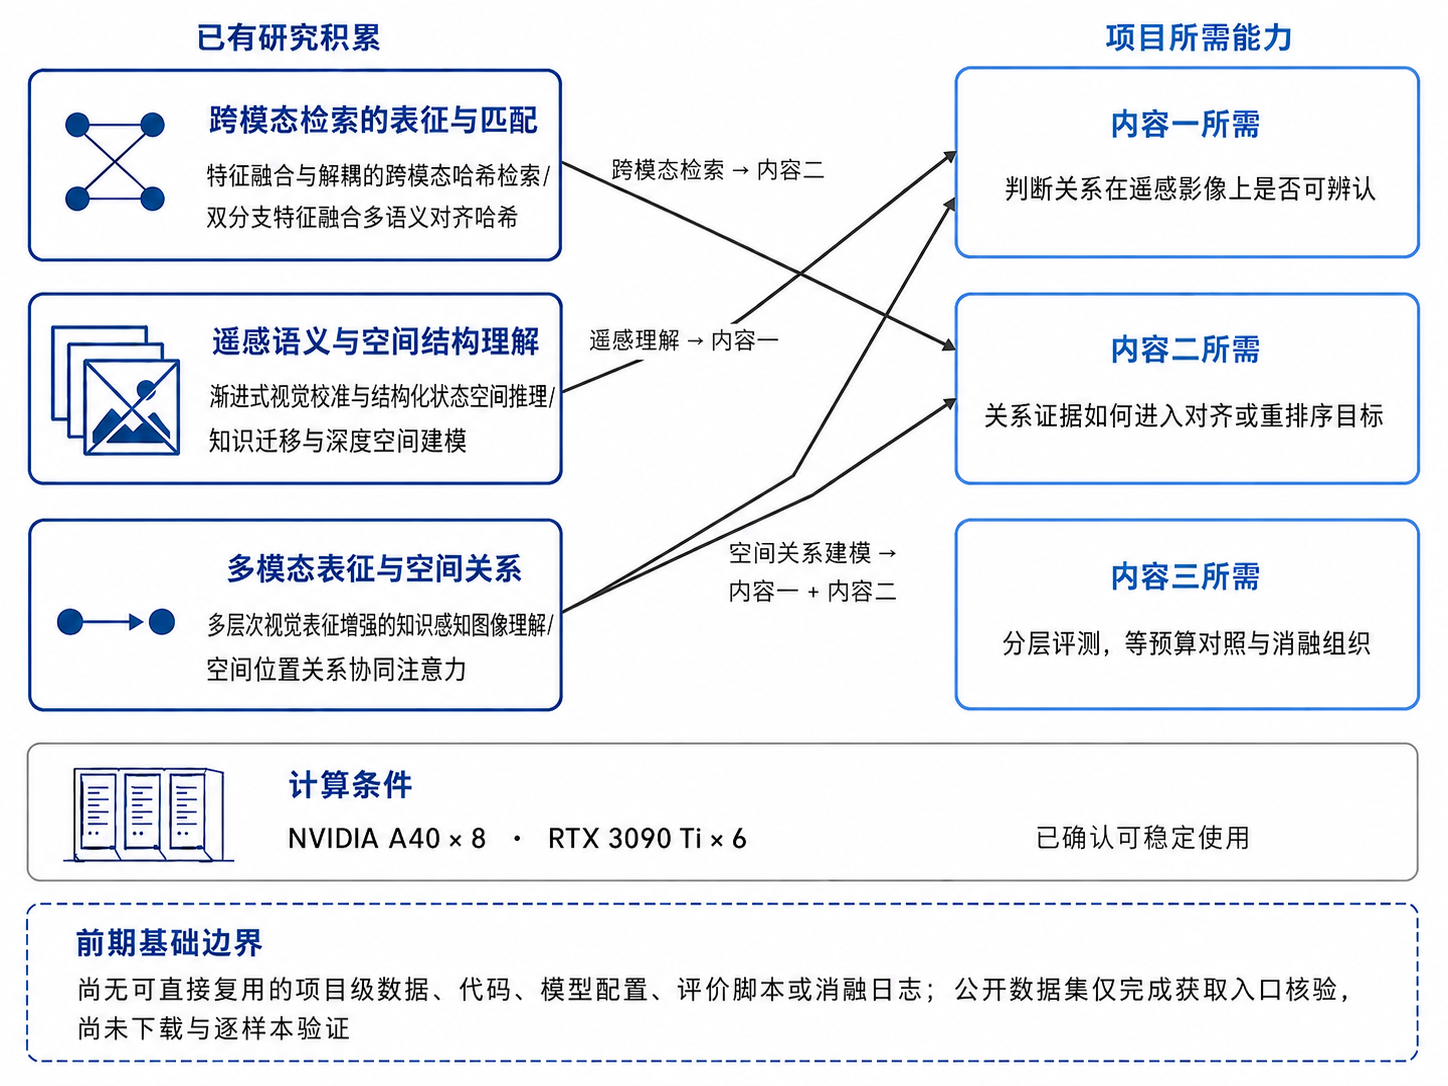
\includegraphics[width=\linewidth]{figures/F12_积累与需求对位-v3.png}
    \caption{申请人积累与项目需求对位。已有成果支撑方法与工程能力，项目专属数据、代码和验证材料仍需在执行期内建立。}
    \label{fig:foundation-mapping}
\end{figure}


\subsubsection{研究风险与应对措施}

本项目的主要风险及应对预案如下。所有预案均以"如实报告、调整定位"为原则，不通过改动评测口径或抽样方式维持既定结论。 三条假说的检验时点、证伪判据与降级路径见图~\ref{fig:falsification}。

% F11: F11_假说证伪.png
\begin{figure}[!htbp]
    \centering
    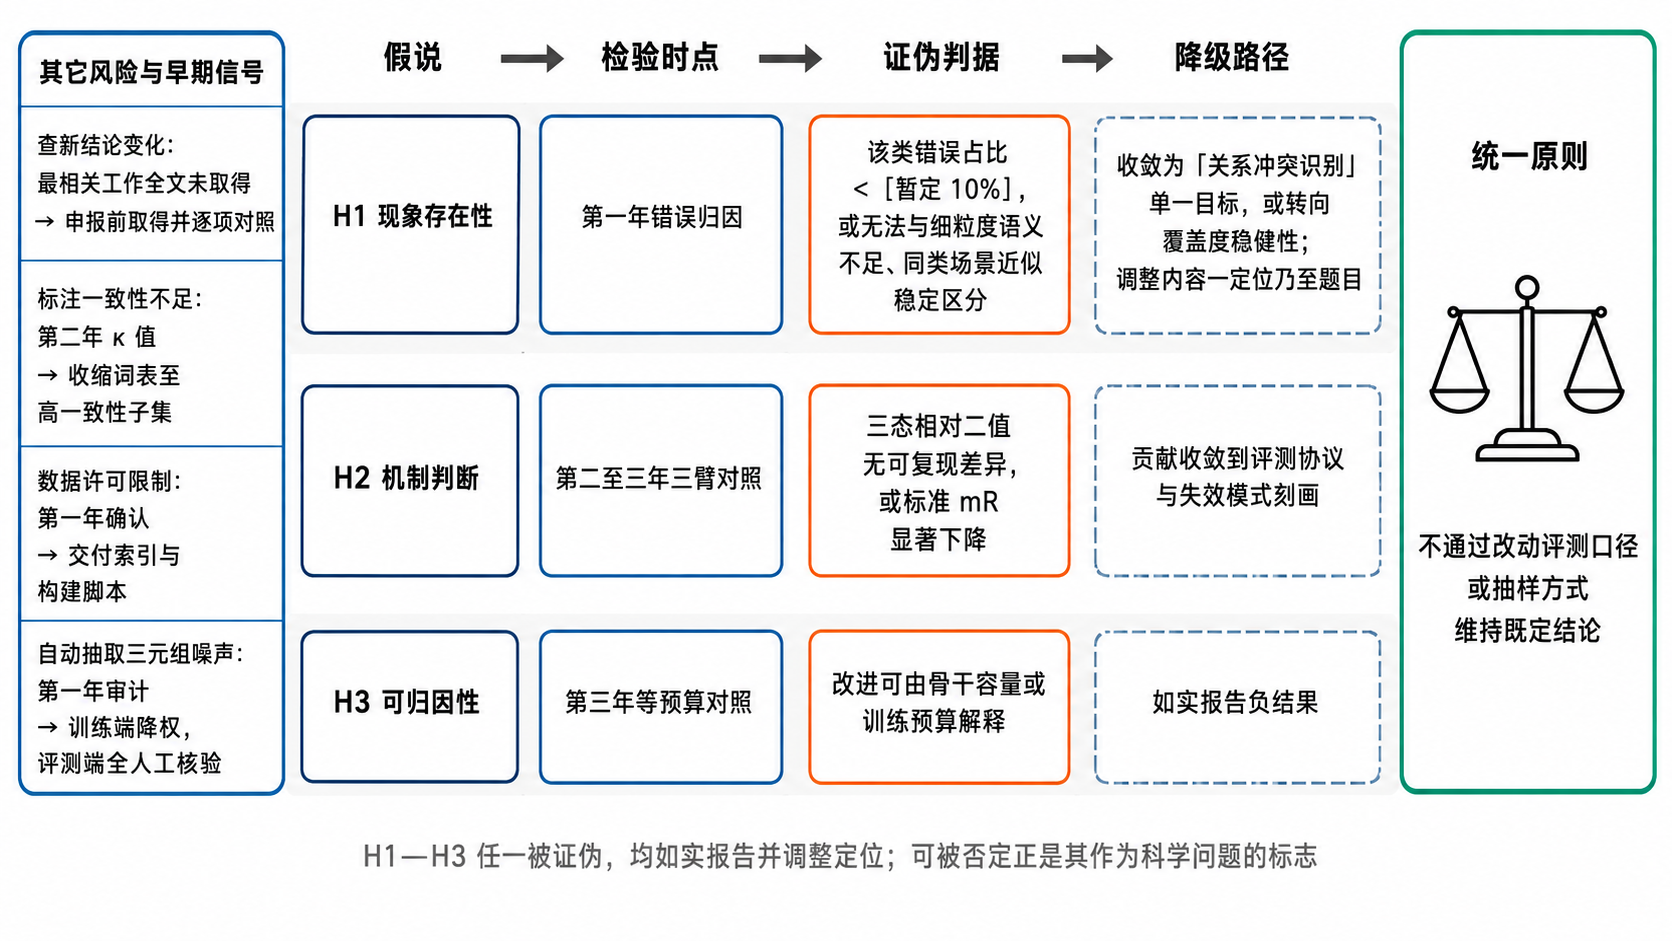
\includegraphics[width=\linewidth]{figures/F11_假说证伪.png}
    \caption{假说、证伪判据与降级路径。H1 阈值为\textbf{【暂定 10\%】}；任一假说被证伪时均如实报告并调整研究定位。}
    \label{fig:falsification}
\end{figure}


\begin{enumerate}
    \item \itemtitlefont{科学假说被证伪的风险。}若第一年的错误归因表明"描述不完备"并非检索失效的重要成因，或该类错误无法与细粒度语义不足、同类场景近似等既有成因稳定区分，则假说 H1 不成立。\textbf{应对}：本项目已预置退出路径——将研究定位调整为"关系冲突识别"这一更窄但仍然成立的目标，或转向描述覆盖度稳健性问题，并相应修改研究内容一的定位。检验安排在第一年完成，正是为了使调整成本可控。这一风险不是方案缺陷，而是可证伪研究的正常组成部分。

    \item \itemtitlefont{查新结论变化的风险。}本项目最相关工作之一为面向遥感图文检索的空间感知实体关系探索\cite{shui2025esrn}，该文全文目前受出版方访问限制尚未取得。若其已包含与本项目三态划分等价的设计，则创新点一需要下调。\textbf{应对}：在正式提交前通过机构订阅或联系作者取得全文并完成逐项对照；若确有重叠，将贡献收敛到评测协议与未知态屏蔽的系统性比较这一仍然成立的部分。本申请对该工作的差异表述已采取保守措辞，未作需要全文支撑的否定断言。

    \item \itemtitlefont{关系标注一致性不足的风险。}三态判定依赖人工核验，若标注者间一致性偏低，评测结论的可信度将受影响。\textbf{应对}：采用双人独立标注加第三人仲裁；一致性不达标的关系类型直接从词表中剔除，而非放宽判据强行保留；"无从判断"一律标记为未知，不强制补成正例或负例。宁可缩小关系词表，也不接受低质量标签。

    \item \itemtitlefont{改进无法归因的风险。}若性能提升可由骨干容量或训练预算解释，则本项目的机制主张不成立。\textbf{应对}：第三年安排等参数量、等训练步数对照实验专门检验；若改进在等预算条件下消失，将如实报告负结果，并把贡献收敛到评测协议与失效模式刻画。

    \item \itemtitlefont{数据许可与进度风险。}第三方数据许可可能不允许再分发影像或派生标注；参与研究生的分工与投入需按申报时点确认。\textbf{应对}：成果交付优先采用数据索引、处理脚本、版本说明与获准发布的派生内容，许可在第一年确认；三项内容虽有先后依赖但可并行推进，内容三的协议设计可与内容一、二同步开展，论文产出安排在第二、三年以留出返修余量。
\end{enumerate}
